% \section{Relazioni di salto}

Si ricavano le condizioni di salto di velocità e sforzo in corrispondenza di superfici di interfaccia.
 Si sottolinea che queste superfici possono essere superfici introdotte dalla modellazione del problema,
 come ad esempio la superficie di separazione tra due fluidi all'interno della quale in generale agisce
 una tensione superficiale o una superficie di discontinuità tangenziale nel caso di fluido non viscoso,
 oppure superfici fittizie.
 
Si parte dai bilanci in forma integrale scritti per un volume in moto arbitrario. I bilanci di massa e quantità di moto
 del volume in moto arbitrario si ottengono dalle regole di derivazione su domini mobili delle funzioni
 $f = \rho$ e $\bm{f} = \rho \bm{u}$,
\begin{equation}
 \frac{d}{dt} \int_{V(t)} f dV 
    = \frac{d}{dt} \int_{v(t)=V(t)} f dv + \oint_{\partial v(t)=\partial V(t)} f(\bm{v}-\bm{w}) \cdot \bm{\hat{n}} ds 
\end{equation}
dove $\bm{u}$ è la velocità del fluido, $\bm{w}$ è la velocità della superficie di discontinuità.

Il billancio integrale viene fatto su un elemento di volume infinitesimo, ``allungato'' nelle direzioni della superficie.
 Quando il volume dell'elemento infinitesimo tende a zero, tende a zero più velocemente dei contributi sulle superfici
 parallele alla superficie di salto.
 
\begin{figure}[h]
\centering
%\captionsetup[subfigure]{labelformat=empty}
\subfloat[][Definizione delle velocità ai due lati dell'elemento infinitesimo e delle dimensioni dello stesso. La velocità 
    della superficie è indicata con $\bm{w}$.]
   {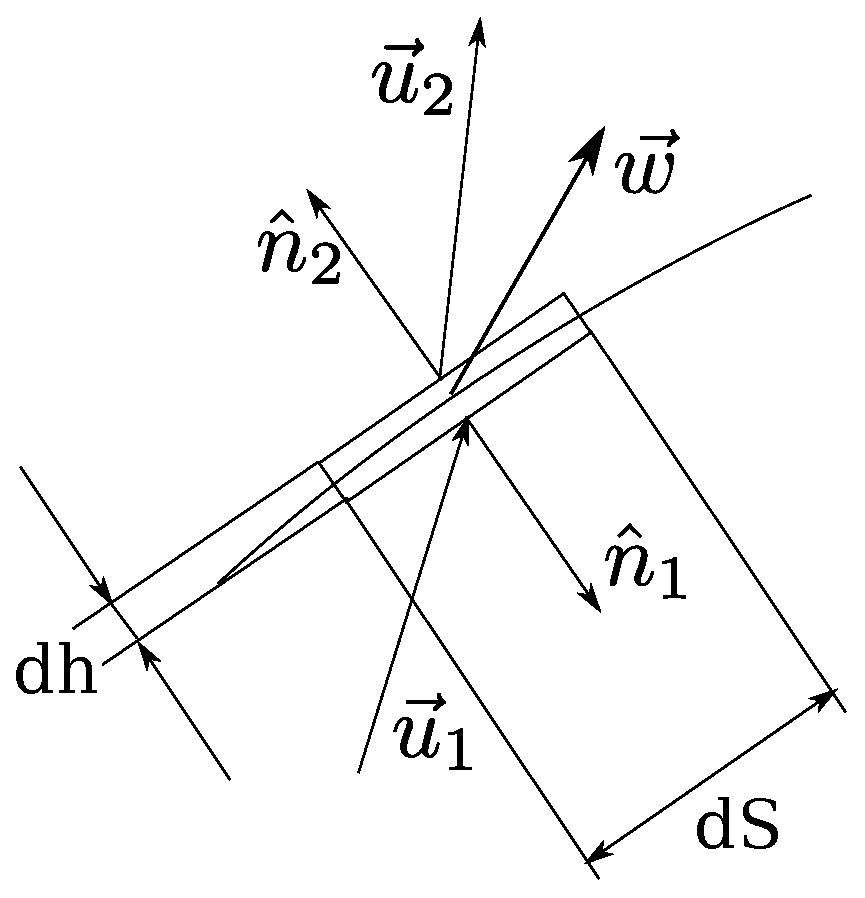
\includegraphics[width=0.30\textwidth]{./fig/elem_velocity.eps}} \qquad \qquad
\subfloat[][Definizione degli sforzi e della tensione superficiale agenti sull'elemento infinitesimo della superficie. ]
   {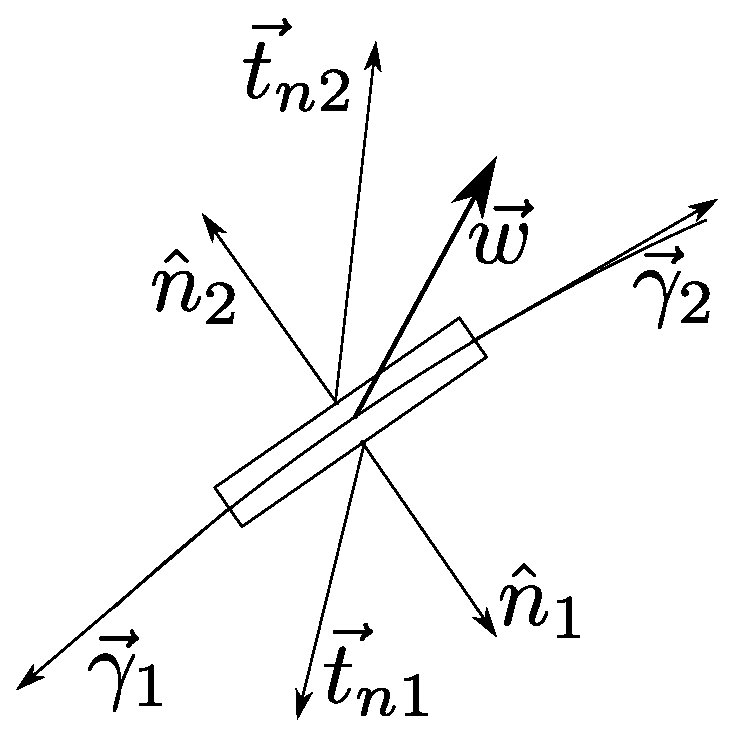
\includegraphics[width=0.30\textwidth]{./fig/elem_stress.eps}}
\end{figure}

L'elemento di volume $dv$ è il parallelepipedo di superfici laterali $dS$, paralleli alla superficie, e basi $dh$ perpendicolari
 alla superficie. Se si ipotizza che le superfici $dh \ll dS$ i contributi nei bilanci dei termini agenti sulle superfici $dh$
 (tranne che nel caso della tensione superficiale, che ha le dimensioni di uno sforzo per una lunghezza) sono trascurabili.


\subsection{Bilancio di massa}
Il bilancio di massa per il volume $dv$  in moto con velocità $\bm{w}$ è
\begin{equation}
 \dfrac{d}{dt}\int_{v} \rho + \oint_{\partial v} \rho (\bm{u} - \bm{w} ) \cdot \bm{\hat{n}} = 0
\end{equation}
Trascurando i contributi di volume e quelli delle superfici $dh$
\begin{equation}
 \rho_1 (\bm{u}_1 - \bm{w} ) \cdot \bm{\hat{n}}_1 dS +  \rho_2 (\bm{u}_2 - \bm{w} ) \cdot \bm{\hat{n}}_2 dS = 0
\end{equation}
dove le normali $\bm{\hat{n}}_1 = \bm{\hat{n}}$ e $\bm{\hat{n}}_2 = -\bm{\hat{n}}$ sono opposte. La quantità tra parentesi è la velocità relativa
 del fluido rispetto alla superficie. Si definisce quindi il flusso di massa $m$ attraverso la superficie.
\begin{equation}
\begin{aligned}
 - m & = \rho_1 (\bm{u}_1 - \bm{w} ) \cdot \bm{\hat{n}} = \rho_2 (\bm{u}_2 - \bm{w} ) \cdot \bm{\hat{n}} \\
   & = \rho_1  \bm{u}_{r1} \cdot \bm{\hat{n}} = \rho_2 \bm{u}_{r2} \cdot \bm{\hat{n}} \\
\end{aligned}
\end{equation}

\noindent
Nel caso di densità uniforme $\rho_1 = \rho_2 = \rho$ si ``conservano'' le componenti normali della velocità relativa e della
 velocità.
\begin{equation}
\begin{aligned}
  \bm{u}_{r1} \cdot \bm{\hat{n}} & = \bm{u}_{r2} \cdot \bm{\hat{n}} \\
  \bm{u}_{1}  \cdot \bm{\hat{n}} & = \bm{u}_{2}  \cdot \bm{\hat{n}} \\
\end{aligned}
\end{equation}


\subsection{Bilancio di quantità di moto}
Il bilancio della quantità di moto per l'elemento $dv$ è
\begin{equation}
 \dfrac{d}{dt}\int_{v} \rho\bm{u} + \oint_{\partial v} \rho \bm{u}(\bm{u} - \bm{w} ) \cdot \bm{\hat{n}} = \oint_{\partial v} \bm{t_n} + \int_{v} \rho \bm{g} + \int_{l} \bm{\gamma}
\end{equation}
avendo incluso anche eventuali termini di tensione superficiale, svolto 
 sulla curva che separa tre sostanze (come ad esempio il ``perimetro''
 del menisco visto nell'esercizio sul capillare: in quel caso la curva
 $l$ separa il liquido, dall'aria, dalle pareti solide del capillare).
Trascurando i termini di volume, il bilancio per l'elemento infinitesimo (per semplicità pensato in 2 dimensioni) è
\begin{equation}
 \rho_1 \bm{u}_1 (\bm{u}_1 - \bm{w})\cdot \bm{\hat{n}}_1 ds + \rho_2 \bm{u}_2 (\bm{u}_2 -\bm{w}) \cdot \bm{\hat{n}}_2 ds =
    \bm{t_{n1}} ds + \bm{\gamma}_1  + \bm{t_{n2}} ds + \bm{\gamma}_2 
\end{equation}
con $\bm{\gamma}_1 = \gamma \bm{\hat{t}_1}$, $\bm{\gamma}_2 = (\gamma + \gamma_{/s} ds) \bm{\hat{t}_2}$. I versori 
 tangenti $\bm{\hat{t}}_1$, $\bm{\hat{t}}_2$ agli estremi dell'elementino di superficie non sono allineati a causa della curvatura della superficie (si
rimanda alla ``dimostrazione'' della legge di Young-Laplace). Si tiene conto di una possibile
 variazione della tensione superficiale. Questa di solito può essere
 dovuta a differenze di temperatura o composizioni chimiche (perchè si
usa il sapone per lavarsi le mani?): si rimanda al 
 simpatico (?) video delle barchette sul fondo del documento della dimostrazione
 della legge di Young-Laplace, nel quale viene usata una ``propulsione a effetto Marangoni'' per barchette di carta. Il contributo della tensione superficiale si può scrivere come
\begin{equation}
 \bm{\gamma}_2 + \bm{\gamma}_1 = (2 \gamma H \bm{\hat{n}} + \bm{\nabla}_2 \gamma )ds
\end{equation}
dove
\begin{itemize}
 \item H è la curvatura media $H = \frac{1}{2}\left(\frac{1}{R_1} + \frac{1}{R_2}\right)$ nel caso tridimensionale, che nel caso bidimensionale
 coincide con $ \frac{1}{2 R}$ (uno dei due raggi di curvatura diventa infinito).
 \item $\bm{\hat{n}}$ è il vettore normale che punta verso i centri di
 curvatura.
 \item $\bm{\nabla}_2$ è il gradiente ristretto alla superficie, tangente ad essa.
\end{itemize}

\noindent
Ricordando la definizione di $m$ e inserendola nel bilancio
\begin{equation}
 m ( \bm{u}_1 - \bm{u}_2 ) =
    \bm{t_{n1}} + \bm{t_{n2}} + 2 \gamma H \bm{\hat{n}} + \bm{\nabla}_2 \gamma
\end{equation}

\noindent
Si analizzano ora alcuni casi particolari:
\begin{itemize}
\item Statica con tensione superficiale. La velocità è nulla ovunque, i vettori di sforzo hanno solo il contributo della pressione
 $\bm{t_n} = -p \bm{\hat{n}}$. Secondo queste ipotesi, non si possono avere contributi tangenziali nemmeno a causa della tensione 
 superficiale e quindi $\gamma$ deve essere uniforme sulla superficie. Nel caso bidimensionale si ricorda che la normale $\bm{\hat{n}}$
 punta verso il centro del cerchio osculatore e coincide quindi con la normale $\bm{\hat{n}}_1$ dell'immagine e il raggio di curvatura $R$ è positivo.
 Il bilancio della quantità di moto si riduce all'equilibrio statico della superficie
 \begin{equation}
   p_1 - p_2 = \frac{\gamma}{R}
 \end{equation}
 Si osserva quindi che la pressione ``interna'' $p_1$ deve essere maggiore di $p_2$.
\item Fluido inviscido, superficie senza tensione superficiale. Il bilancio si riduce a 
\begin{equation}
  m ( \bm{u}_1 - \bm{u}_2 ) = - (p_1 - p_2) \bm{\hat{n}}
\end{equation}
\item Fluido inviscido, superficie senza tensione superficiale, densità uniforme. Si è visto come la 
  velocità (e le velocità relative) normali alla superficie devono essere uguali da entrambe le parti
  della superficie. %Se la superficie è una superficie materiale, la velocità della superficie coincide
%  con quella del fluido e quindi la velocità relativa è nulla ed $m = 0$.
%  Risulta quindi che non ci può essere salto di pressione attraverso una tale superficie (questo è quello che significa
%  l'ipotesi espressa in termini pittoreschi di ``scia scarica'' nell'aerodinamica a potenziale).
%  \begin{equation}
%    p_1 = p_2
%  \end{equation}
  Se si ipotizza che la superifice non sia attraversata da flusso di massa (si impone che la componente normale della velocità relativa sia nulla,
  non la velocità relativa nel suo complesso). In questo caso non è possibile trovare una relazione 
  di salto per la velocità tangenziale (o almeno questo non è possibile se non si aggiungono altre ipotesi o altre equazioni \dots vedremo 
  un caso semplificato applicando il teorema di Bernoulli a un problema aerodinamico bidimensionale stazionario \dots):
  poichè $m=0$ la superficie è ``scarica'' (capiterà nei prossimi corsi di sentir parlare o aver direttamente a che fare con ``
  l'ipotesi di scia scarica'': questa non dovrà quindi essere una novità o una sorpresa in futuro)
  \begin{equation}
    p_1 = p_2
  \end{equation}
  ma non si riesce a ricavare nessuna informazione dalla componente tangenziale
  dell'equazione poichè è un'identità $0=0$ a prescindere dal valore di $( \bm{u}_1 - \bm{u}_2 )\cdot \bm{\hat{t}}$. Attraverso tale superficie
  (di spessore nullo) ci può essere un salto finito di velocità tangenziale: in questo caso la superficie è una superficie di vorticità infinita
\end{itemize}

\noindent
L'ultimo caso particolare verrà utilizzato in qualche esercizio in cui un dominio occupato da un fluido può essere suddiviso in un sottodominio 
 nel quale è valido il teorema di Bernoulli (in qualche forma \dots) e in un sottodominio dove sono valide le relazioni della statica: le condizioni
 di salto serviranno a far comunicare tra di loro i due sottodomini (e a risolvere correttamente l'esercizio).

\subsection{Bilancio di energia}
Non verrà detto nulla sulle relazioni di salto delle altre quantità \dots

